
\chapter{\elemMatDetIITitle}\label{elementarydeterminantsII}

In section~\ref{elementarydeterminants}, we saw the definition of the determinant and derived an elementary matrix that exchanges two rows of a matrix.  Next, we need to find elementary matrices corresponding to the other two row operations; multiplying a row by a scalar, and adding a multiple of one row to another.  As a consequence, we will derive some important properties of the determinant.

Consider $M=\colvec{R^1 \\ \vdots \\ R^n }$, where $R^i$ are row vectors.  Let $R^i(\lambda)$ be the identity matrix, with the $i$th diagonal entry replaced by $\lambda$, not to be confused with the row vectors. {\it I.e.}
$$
R^i(\lambda)=
\begin{pmatrix}
1 & & & & \\
  & \ddots & & & \\
  & & \lambda & & \\
  & & & \ddots & \\
  & & & & 1 \\
\end{pmatrix}
\, .$$
Then:

\[
M'=R^i(\lambda)M=\colvec{R^1 \\ \vdots \\ \lambda R^i \\ \vdots \\ R^n }
\]
What effect does multiplication by $R^i(\lambda)$ have on the determinant?

\begin{eqnarray*}
\det M' & = & \sum_{\sigma} \text{sgn}(\sigma) m^1_{\sigma(1)}\cdots \lambda m^i_{\sigma(i)} \cdots m^n_{\sigma(n)} \\
& = & \lambda \sum_{\sigma} \text{sgn}(\sigma) m^1_{\sigma(1)}\cdots m^i_{\sigma(i)} \cdots m^n_{\sigma(n)} \\
& = & \lambda \det M
\end{eqnarray*}
Thus, multiplying a row by $\lambda$ multiplies the determinant by $\lambda$.
{\it I.e.,} $$\det R^i(\lambda) M = \lambda \det M\, .$$


\begin{figure}
\begin{center}
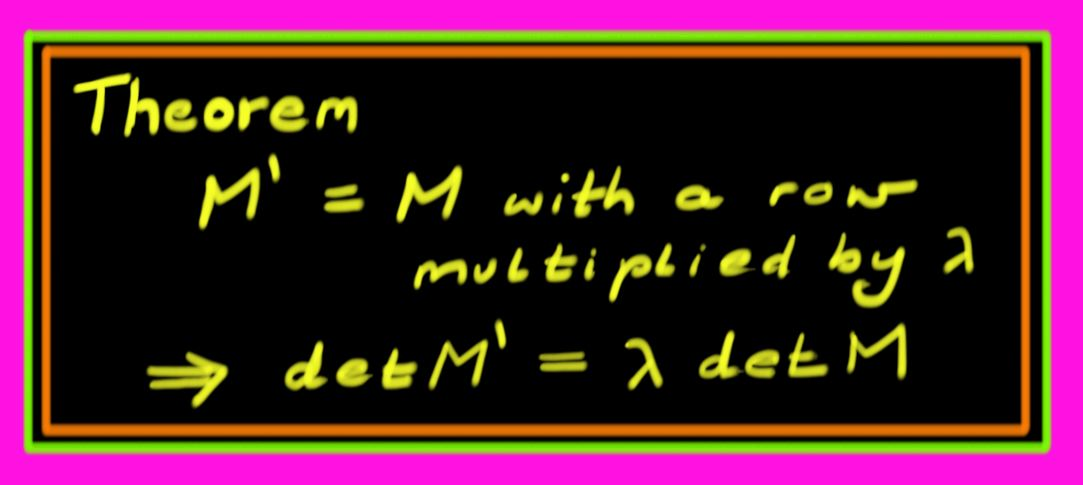
\includegraphics[scale=.27]{\elemMatDetIIPath/row_mult_thm.jpg}
\end{center}
\end{figure}


Since $R^i(\lambda)$ is just the identity matrix with a single row multiplied by $\lambda$, then by the above rule, the determinant of $R^i(\lambda)$ is $\lambda$.  Thus:

\[
\det R^i(\lambda) = \det \begin{pmatrix}
1 & & & & \\
  & \ddots & & & \\
  & & \lambda & & \\
  & & & \ddots & \\
  & & & & 1 \\
\end{pmatrix} = \lambda
\]

The final row operation is adding $\lambda R^j$ to $R^i$.  This is done with the matrix~$S^i_j(\lambda)$, which is an identity matrix but with a $\lambda$ in the $i,j$ position.

\[
S^i_j(\lambda) = \begin{pmatrix}
1 & 	& 	& 	& & & 	\\
  & \ddots & 	&	& & &	\\
  & 	& 1 	& 	& \lambda & &	\\
  & 	& 	& \ddots & & &	\\
  & 	& 	& 	& 1 & & 	\\
  & 	& 	& 	& 	& \ddots & 	\\
  & 	& 	& 	& 	& 	 & 1	\\
\end{pmatrix}
\]
Then multiplying $S^i_j(\lambda)$ by $M$ gives the following:

\[
\begin{pmatrix}
1 & 	& 	& 	& & & 	\\
  & \ddots & 	&	& & &	\\
  & 	& 1 	& 	& \lambda & &	\\
  & 	& 	& \ddots & & &	\\
  & 	& 	& 	& 1 & & 	\\
  & 	& 	& 	& 	& \ddots & 	\\
  & 	& 	& 	& 	& 	 & 1	\\
\end{pmatrix}\colvec{\\ \vdots \\ R^i \\ \vdots \\ R^j \\ \vdots\\ \\}
=
\colvec{\\ \vdots \\ R^i +\lambda R^j \\ \vdots \\ R^j \\ \vdots\\ \\ }
\]
What is the effect of multiplying by $S^i_j(\lambda)$ on the determinant?  Let $M'=S^i_j(\lambda)M$, and let $M''$ be the matrix $M$ but with $R^i$ replaced by $R^j$.

\begin{eqnarray*}
\det M' & = & \sum_{\sigma} \text{sgn}(\sigma) m^1_{\sigma(1)}\cdots (m^i_{\sigma(i)}+ \lambda m^j_{\sigma(j)}) \cdots m^n_{\sigma(n)} \\
& = & \sum_{\sigma} \text{sgn}(\sigma) m^1_{\sigma(1)}\cdots m^i_{\sigma(i)} \cdots m^n_{\sigma(n)} \\
&   & \qquad + \sum_{\sigma} \text{sgn}(\sigma) m^1_{\sigma(1)}\cdots \lambda m^j_{\sigma(j)} \cdots m^j_{\sigma(j)} \cdots m^n_{\sigma(n)} \\
& = & \det M + \lambda \det M''
\end{eqnarray*}
Since $M''$ has two identical rows, its determinant is $0$.  Then $$\det S^i_j(\lambda)M = \det M\, .$$
Notice that if $M$ is the identity matrix, then we have $$\det S^i_j(\lambda) = \det (S^i_j(\lambda)I) = \det I = 1\, .$$

\begin{figure}
\begin{center}
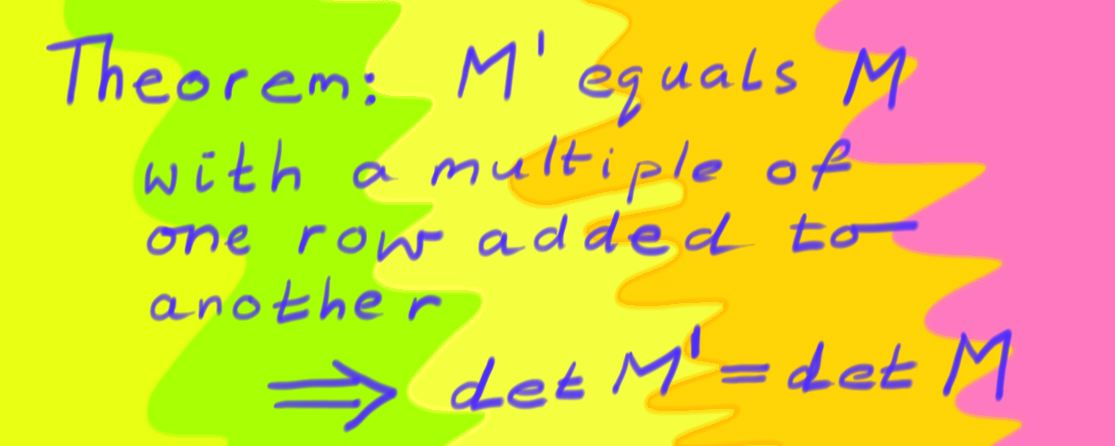
\includegraphics[scale=.27]{\elemMatDetIIPath/row_addition_thm.jpg}
\end{center}
\end{figure}

We now have elementary matrices associated to each of the row operations.

\[
\begin{array}{cccc}
E^i_j &=& I \text{ with rows $i,j$ swapped;} &\det E^i_j=-1 \\[3mm]
R^i(\lambda) &=& I \text{ with $\lambda$ in position $i,i$;} 
	&\det R^i(\lambda)=\lambda \\[3mm]
S^i_j(\lambda) &=& I \text{ with $\lambda$ in position $i,j$;} 
	&\det S^i_j(\lambda)=1 \\[3mm]
\end{array}
\]
\videoscriptlink{elementary_matrices_and_determinants_ii_dets.mp4}{Elementary Determinants}{scripts_elementary_matrices_determinants_ii_dets}
We have also proved the following theorem along the way:

\begin{theorem}
If $E$ is \emph{any} of the elementary matrices $E^i_j, R^i(\lambda), S^i_j(\lambda)$, then $\det(EM)=\det E \det M$.
\end{theorem}

%\href{\webworkurl ReadingHomework13/1/}{Reading homework: problem 13.1}
\reading{13}{1}


\begin{center}
\hspace{3mm}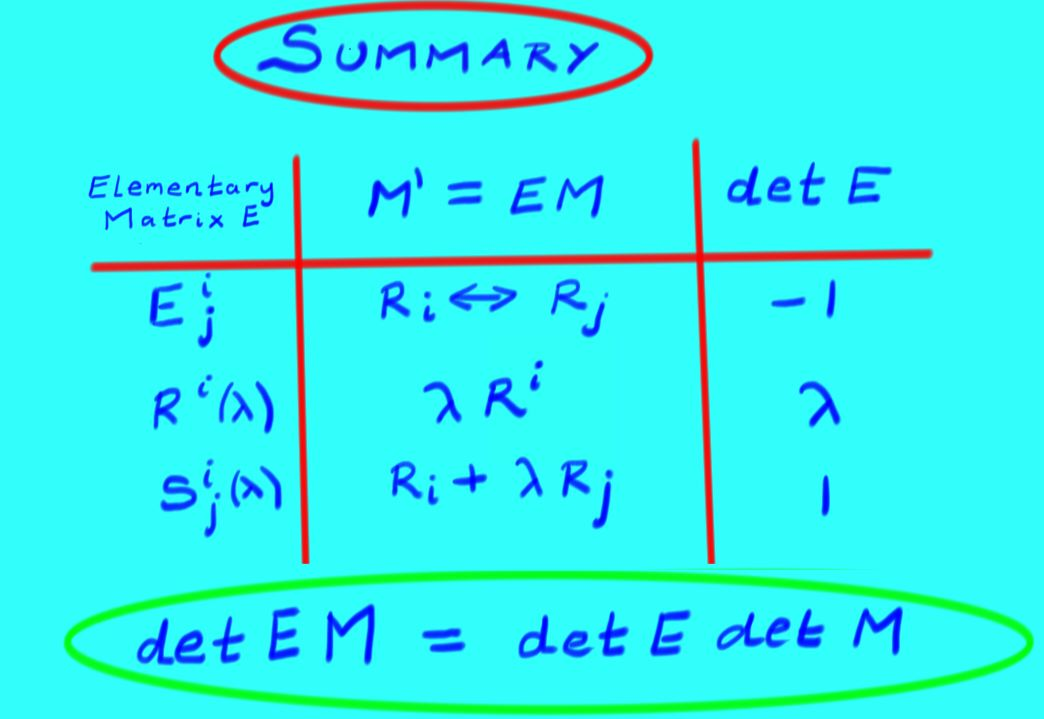
\includegraphics[scale=.27]{\elemMatDetIIPath/summary.jpg}
\end{center}


We have seen that any matrix $M$ can be put into reduced row echelon form via a sequence of row operations, and we have seen that any row operation can be emulated with left matrix multiplication by an elementary matrix.  Suppose that $\rref(M)$ is the reduced row echelon form of $M$.  Then $\rref(M)=E_1E_2\cdots E_kM$ where each $E_i$ is an elementary matrix.

What is the determinant of a square matrix in reduced row echelon form?  
\begin{itemize}
\item If $M$ is not invertible, then some row of $\rref(M)$ contains only zeros.  Then we can multiply the zero row by any constant $\lambda$ without changing~$M$; by our previous observation, this scales the determinant of $M$ by $\lambda$.  Thus, if $M$ is not invertible, $\det \rref(M)=\lambda \det \rref(M)$, and so $\det \rref(M)=0$.  

\item Otherwise, every row of $\rref(M)$ has a pivot on the diagonal; since $M$ is square, this means that $\rref(M)$ is the identity matrix.  Then if $M$ is invertible, $\det \rref(M)=1$.

\item Additionally, notice that $\det \rref(M) = \det (E_1E_2\cdots E_kM)$.  Then by the theorem above, $\det \rref(M)=\det (E_1) \cdots \det (E_k) \det M$.  Since each $E_i$ has non-zero determinant, then $\det \rref(M)=0$ if and only if $\det M=0$.
\end{itemize}
Then we have shown:

\begin{theorem}
\label{detinvertible}
For any square matrix $M$, $\det M\neq 0$ if and only if $M$ is invertible.
\end{theorem}
Since we know the determinants of the elementary matrices, we can immediately obtain the following:


\videoscriptlink{elementary_matrices_ii_inverses_determinants.mp4}{Determinants and Inverses}{scripts_elementary_matrices_determinants_ii_inverses}

\begin{figure}
\begin{center}
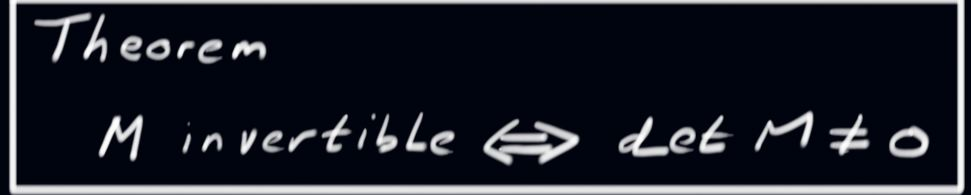
\includegraphics[scale=.27]{\elemMatDetIIPath/theorem_invertible.jpg}
\end{center}
\end{figure}

\begin{corollary}
Any elementary matrix $E^i_j, R^i(\lambda), S^i_j(\lambda)$ is invertible, except for $R^i(0)$.  In fact, the inverse of an elementary matrix is another elementary matrix.
\end{corollary}


To obtain one last important result, suppose that $M$ and $N$ are square $n\times n$ matrices, with reduced row echelon forms such that, for elementary matrices  $E_i$ and $F_i$, $$M=E_1E_2\cdots E_k \, \rref(M)\, ,$$ and  $$N=F_1F_2\cdots F_l \, \rref(N)\, .$$  If $\rref(M)$ is the identity matrix ({\it i.e.}, $M$ is invertible), then:

\begin{eqnarray*}
\det (MN) & = & \det (E_1E_2\cdots E_k\,  \rref(M) F_1F_2\cdots F_l \, \rref(N) )\\
& = & \det (E_1E_2\cdots E_k I F_1F_2\cdots F_l\,  \rref(N) )\\
& = & \det (E_1) \cdots \det(E_k)\det(I)\det(F_1)\cdots\det(F_l)\det(\rref(N)\\
& = & \det(M)\det(N)
\end{eqnarray*}
Otherwise, $M$ is not invertible, and $\det M=0=\det 
\rref(M)$.  Then there exists a row of zeros in $
\rref(M)$, so $R^n(\lambda)
\rref(M)=
\rref(M)$.  Then:
\begin{eqnarray*}
\det (MN) & = & \det (E_1E_2\cdots E_k 
\, \rref(M) N )\\
& = & \det (E_1E_2\cdots E_k 
\, \rref(M) N )\\
& = & \det (E_1) \cdots \det(E_k)\det( 
\rref(M)N)\\
& = & \det (E_1) \cdots \det(E_k)\det( R^n(\lambda) 
\, \rref(M)N)\\
& = & \det (E_1) \cdots \det(E_k)\lambda \det( 
\rref(M)N)\\
& = & \lambda \det (MN)
\end{eqnarray*}
Which implies that $\det (MN)=0=\det M \det N$.

Thus we have shown that for {\it any} matrices $M$ and $N$, 
\label{detmultiplicative}
\[
\det (MN) = \det M \det N
\]
This result is {\it extremely important}; do not forget it!

\videoscriptlink{elementary_matrices_determinant_ii_product.mp4}{Alternative proof}{scripts_elementary_matrices_determinants_ii_product}

\begin{figure}
\begin{center}

\includegraphics[scale=.27]{\elemMatDetIIPath/detMN.jpg}
\end{center}
\end{figure}

%\href{\webworkurl ReadingHomework13/2/}{Reading homework: problem 13.2}
\reading{13}{2}

%\section*{References}
%Hefferon, Chapter Four, Section I.1 and I.3
%\\
%Beezer, Chapter D, Section DM, Subsection EM
%\\
%Beezer, Chapter D, Section PDM
%\\
%Wikipedia:
%\begin{itemize}
%\item \href{http://en.wikipedia.org/wiki/Determinant}{Determinant}
%\item \href{http://en.wikipedia.org/wiki/Elementary_matrix}{Elementary Matrix}
%\end{itemize}

\section{Review Problems}




\begin{enumerate}

\item Let $D=\begin{pmatrix}
\lambda_1 & \mc0 \\
\mc0 & \lambda_2 \\
\end{pmatrix}$.
\begin{enumerate}
\item Write $D$ in terms of the vectors $e_1$ and $e_2$, and their transposes.
\item Suppose $P=\begin{pmatrix}
a & b \\
c & d \\
\end{pmatrix}$ is invertible.  Show that $D$ is similar to
\[
M=\frac{1}{ad-bc}\begin{pmatrix}
\lambda_1ad-\lambda_2bc & -(\lambda_1-\lambda_2)ab \\[1mm]
(\lambda_1-\lambda_2)cd & -\lambda_1bc + \lambda_2ad
\end{pmatrix}.
\]
\item Suppose the vectors $\rowvec{a,b}$ and $\rowvec{c,d}$ are orthogonal.  What can you say about $M$ in this case? (Hint: think about what \(M^T\) is equal to.)
\end{enumerate}

\phantomnewpage

\item \label{orthogprob} Suppose $S=\{v_1, \ldots, v_n \}$ is an \emph{orthogonal} (not orthonormal) basis for~$\Re^n$.  Then we can write any vector $v$ as $v=\sum_ic^iv_i$ for some constants $c^i$.  Find a formula for the constants $c^i$ in terms of $v$ and the vectors in~$S$.

\Videoscriptlink{orthonormal_bases_hint.mp4}{Hint}{scripts_orthonormal_bases_hint}
\phantomnewpage

\item \label{orthogprojprob} Let $u,v$ be linearly independent vectors in $\Re^3$, and $P=\spa \{ u,v\}$ be the plane spanned by $u$ and $v$.  
\begin{enumerate}
\item Is the vector $v^\bot := v-\frac{u\cdot v}{u\cdot u}u$ in the plane $P$?
\item  What is the (cosine of the) angle between $v^\bot$ and $u$?
\item %Given your solution to the above, 
How can you find a third vector perpendicular to both $u$ and $v^\bot$?
\item  Construct an orthonormal basis for $\Re^3$ from $u$ and $v$.
\item  Test your abstract formul\ae\ starting with 
\[
u=\rowvec{1 , 2 , 0} \text{ and } v=\rowvec{0 , 1 , 1}.
\]
\end{enumerate}

\Videoscriptlink{orthonormal_bases_hint3.mp4}{Hint}{scripts_orthonormal_bases_hint3}

\phantomnewpage



\item Find an orthonormal  basis for $\Re^4$ which includes $(1,1,1,1)$ using the following procedure:\\
\begin{enumerate} 
\item Pick a vector perpendicular to the vector 
$$v_1 =\colvec{1\\1\\1\\1}$$ from the solution set of the matrix equation $$v_1^Tx=0\, .$$ Pick the vector $v_2$ obtained from the standard Gaussian elimination procedure which is the coefficient of $x_2$.
\item Pick a vector perpendicular to both $v_1$ and $v_2$ from the solutions set of the matrix equation $$\colvec{v_1^T\\[1mm]v_2^T}x=0\, .$$ Pick the vector $v_3$ obtained from the standard Gaussian elimination procedure with $x_3$ as the coefficient. 
\item Pick a vector perpendicular to $v_1,v_2,$ and $v_3$ from the solution set of the matrix equation $$\colvec{v_1^T\\[1mm]v_2^T\\[1mm]v_3^T}x=0\, .$$  Pick the vector $v_4$ obtained from the standard Gaussian elimination procedure with $x_3$ as the coefficient. 
\item Normalize the four vectors obtained   above.
\end{enumerate}


\item Use the inner product $$f\cdot g := \int_0^1 f(x)g(x)dx$$  on the vector space $V={\rm span} \{1,x,x^2,x^3\}$ to perform the Gram-Schmidt procedure on the set of vectors $\{1,x,x^2,x^3\}$. 

\item Use the inner product $$f\cdot g := \int_0^{2\pi} f(x)g(x)dx$$  on the vector space $V={\rm span} \{\sin(x),\sin(2x),\sin(3x) \}$ to perform the Gram-Schmidt procedure on the set of vectors $\{\sin(x),\sin(2x),\sin(3x) \}$. \\
Try to build an orthonormal basis for the vector space $$\spa \{ \sin(nx)~| ~n\in \N \}\, .$$
%What do you suspect about the vector space $\spa \{ \sin(nx)~| ~n\in \N \}$?\\
%What do you suspect about the vector space $\spa \{ \sin(ax)~|~ a \in \Re \}$?
\item 
\begin{enumerate}
\item
Show that if $Q$ is an orthogonal $n\times n$ matrix, then $$u\dotprod v = (Qu)\dotprod (Qv)\, ,$$ for any $u,v\in \Re^n$. That is, $Q$ preserves the inner product. 
\item Does $Q$ preserve the outer product? 
\item  If the set of vectors $\{ u_1,\dots,u_n\}$ is orthonormal and $\{ \lambda_1,\cdots,\lambda_n\}$ is a set of numbers, 
then what are the eigenvalues and eigenvectors of the matrix
$M=\sum_{i=1}^n \lambda_i u_i u_i^T$? 
\item How would the eigenvectors and eigenvalues of this matrix change if we replaced  $\{ u_1,\dots,u_n\}$ by $\{ Qu_1,\dots,Q u_n\}$?
\end{enumerate}


\item Carefully write out the Gram-Schmidt procedure for the set of vectors 
$$\left\{ \colvec{1\\1\\1}, \colvec{1\\-1\\1}, \colvec{1\\1\\-1} \right\} \, .$$ Is it possible to rescale the second vector obtained in the procedure to a vector with integer components? 


\item 
\label{basisortho}
\begin{enumerate}
\item Suppose $u$ and $v$ are linearly independent.  Show that $u$ and $v^\perp$ are also linearly independent.  Explain why $\{u, v^\perp\}$ is a basis for $\spa \{u,v\}$.



\Videoscriptlink{gram_schmidt_and_orthogonal_complements_hint.mp4}{Hint}{gram_schmidt_and_orthogonal_complements_hint}

\item Repeat the previous problem, but with three independent vectors $u,v,w$
 where $v^\perp$ and $w^\perp$ are as defined by the Gram-Schmidt procedure. 
\end{enumerate}

\phantomnewpage


\item \label{QRprob} Find the $QR$ factorization of
$$
M=\begin{pmatrix}1&0&\phantom{\!-}2\\-1&2&0\\-1&-2&2
\end{pmatrix}\, .
$$

\phantomnewpage

\item Given any three vectors $u,v,w$, when do $v^\perp$ or $w^\perp$ of the Gram--Schmidt procedure vanish?

\phantomnewpage

\item For $U$ a subspace of $W$, use the subspace theorem to check that $U^\perp$ is a subspace of $W$.

\phantomnewpage


\phantomnewpage

\item %(Extra Credit) 
Let $S_n$ and $A_n$ define the space of $n \times n$ symmetric and anti-symmetric matrices, respectively. These are subspaces of the vector space $M^n_n$ of all $n\times n$ matrices. What is $\dim M^n_n$, $\dim S_n$, and $\dim A_n$? Show that $M^n_n = S_n + A_n$. Define an inner product on square matrices
$$
M\cdot N ={\rm tr} MN\, .
$$
Is $A_n^{\perp}=S_n$? Is $M^n_n = S_n \oplus A_n$?

%\emph{Hint: Note that $\dim S_n = \dim U_n$ where $U_n$ is the vector space of all $n \times n$ upper triangular matrices, and also note that $\dim A_n = \dim \widetilde{U}_n$ where $\widetilde{U}_n$ is the vector space of all strictly $n \times n$ upper triangular matrices (\emph{i.e.} the diagonal entries are all 0).}

\item The vector space $V={\rm span} \{ \sin(t),\sin(2t), \sin(3t) , \sin(3t)\}$ has an inner product: 
$$f\cdot g:=\int _0^{2\pi}f(t)g(t) dt\, .$$ Find the orthogonal compliment to $U={\rm span} \{ \sin(t)+\sin(2t) \}$ in $V$. Express $\sin(t)-\sin(2t)$ as  the sum of vectors from $U$ and $U^\perp$.

\end{enumerate}

\phantomnewpage

\newpage



